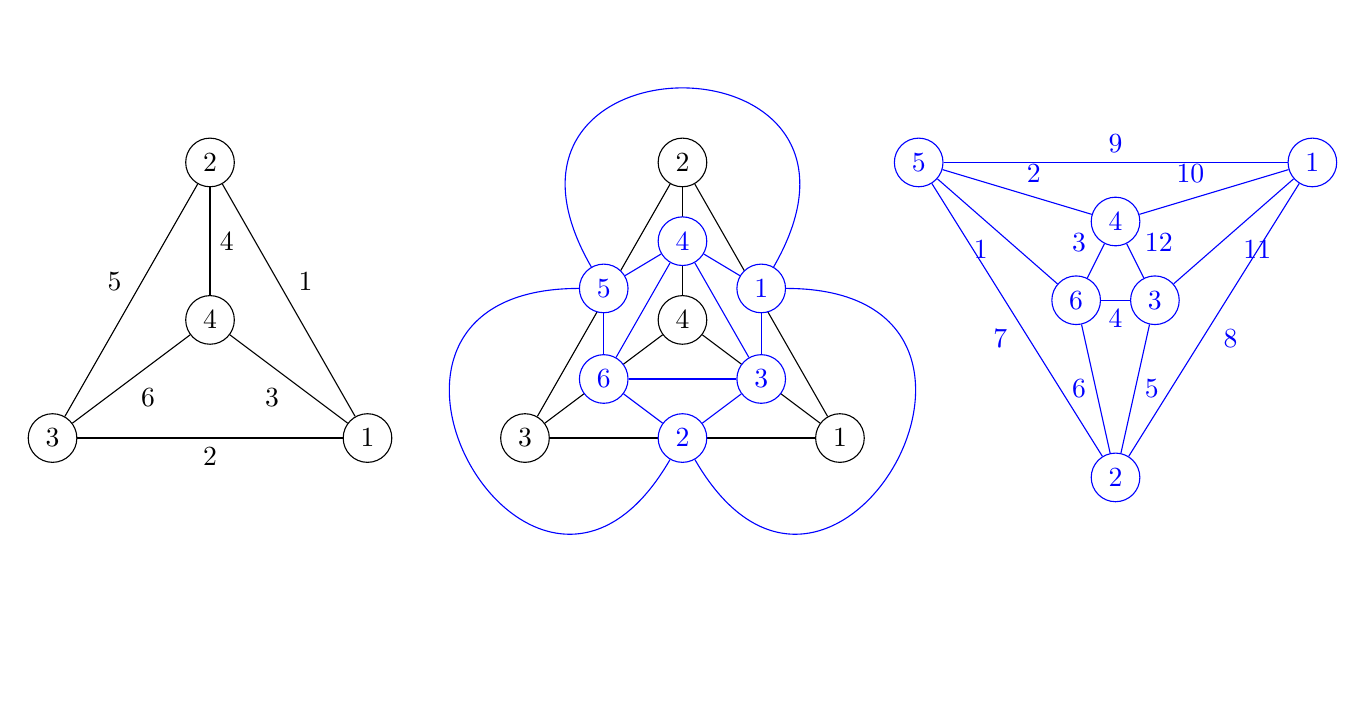
\begin{tikzpicture}
	\begin{scope}[xshift=0cm, yshift=2cm, scale=0.5]
		\node[circle, draw] (1) at (4, -3) {1};
		\node[circle, draw] (2) at (0, 4) {2};
		\node[circle, draw] (3) at (-4, -3) {3};
		\node[circle, draw] (4) at (0, 0) {4};
	
		\draw[draw] (1) -- node[above right] {1} (2);
		\draw[draw] (1) -- node[below] {2} (3);
		\draw[draw] (1) -- node[below left] {3} (4);
		\draw[draw] (2) -- node[right] {4} (4);
		\draw[draw] (2) -- node[above left] {5} (3);
		\draw[draw] (3) -- node[below right] {6} (4);
	\end{scope}

	\begin{scope}[xshift=6cm, yshift=2cm, scale=0.5]
		\node[circle, draw] (g1) at (4, -3) {1};
		\node[circle, draw] (g2) at (0, 4) {2};
		\node[circle, draw] (g3) at (-4, -3) {3};
		\node[circle, draw] (g4) at (0, 0) {4};
	
		\draw[draw] (g1) -- node[above right] {} (g2);
		\draw[draw] (g1) -- node[below] {} (g3);
		\draw[draw] (g1) -- node[below left] {} (g4);
		\draw[draw] (g2) -- node[right] {} (g4);
		\draw[draw] (g2) -- node[above left] {} (g3);
		\draw[draw] (g3) -- node[below right] {} (g4);

		\node[circle, blue, draw, fill=white] (m1) at (2, 0.8) {1};
		\node[circle, blue, draw, fill=white] (m2) at (0, -3) {2};
		\node[circle, blue, draw, fill=white] (m3) at (2, -1.5) {3};
		\node[circle, blue, draw, fill=white] (m4) at (0, 2) {4};
		\node[circle, blue, draw, fill=white] (m5) at (-2, 0.8) {5};
		\node[circle, blue, draw, fill=white] (m6) at (-2, -1.5) {6};

		\draw[draw, blue] (m5) -- node[below left] {} (m6);
		\draw[draw, blue] (m5) -- node[above right] {} (m4);
		\draw[draw, blue] (m4) -- node[above left] {} (m6);
		\draw[draw, blue] (m3) -- node[below] {} (m6);
		\draw[draw, blue] (m3) -- node[right] {} (m2);
		\draw[draw, blue] (m6) -- node[left] {} (m2);
		\draw[draw, blue] (m2) to[in=180,out=-120,loop, min distance=7cm] node[below left] {} (m5);
		\draw[draw, blue] (m1) to[in=-60,out=0,loop, min distance=7cm] node[below right] {} (m2);
		\draw[draw, blue] (m1) to[in=120,out=60,loop, min distance=7cm] node[above] {} (m5);
		\draw[draw, blue] (m1) -- node[above left] {} (m4);
		\draw[draw, blue] (m1) -- node[below right] {} (m3);
		\draw[draw, blue] (m4) -- node[above right] {} (m3);
	\end{scope}

	\begin{scope}[xshift=10cm, yshift=4cm, scale=0.5]
		\node[circle, blue, draw] (1) at (8, -0) {1};
		\node[circle, blue, draw] (2) at (3, -8) {2};
		\node[circle, blue, draw] (3) at (4, -3.5) {3};
		\node[circle, blue, draw] (4) at (3, -1.5) {4};
		\node[circle, blue, draw] (5) at (-2, -0) {5};
		\node[circle, blue, draw] (6) at (2, -3.5) {6};
	
		% Draw the edges between nodes with labels
		\draw[draw, blue] (5) -- node[below left] {1} (6);
		\draw[draw, blue] (5) -- node[above right] {2} (4);
		\draw[draw, blue] (4) -- node[above left] {3} (6);
		\draw[draw, blue] (3) -- node[below] {4} (6);
		\draw[draw, blue] (3) -- node[right] {5} (2);
		\draw[draw, blue] (6) -- node[left] {6} (2);
		\draw[draw, blue] (2) -- node[below left] {7} (5);
		\draw[draw, blue] (1) -- node[below right] {8} (2);
		\draw[draw, blue] (1) -- node[above] {9} (5);
		\draw[draw, blue] (1) -- node[above left] {10} (4);
		\draw[draw, blue] (1) -- node[below right] {11} (3);
		\draw[draw, blue] (4) -- node[above right] {12} (3);
	\end{scope}
\end{tikzpicture}
